\documentclass{beamer} 

% Michael Maier, 2013.
% CC-BY-SA

\usepackage[utf8]{inputenc}
\usepackage[ngerman]{babel}

\title{OpenStreetMap - Die freie Wiki-Weltkarte} 
\author{Michael Maier \textless Michael.Maier@student.tugraz.at\textgreater} 
\date{20. April 2013} 

\usetheme{Antibes}

\hypersetup{colorlinks=true,urlcolor=blue,linkcolor=white}

%\usebackgroundtemplatei{
%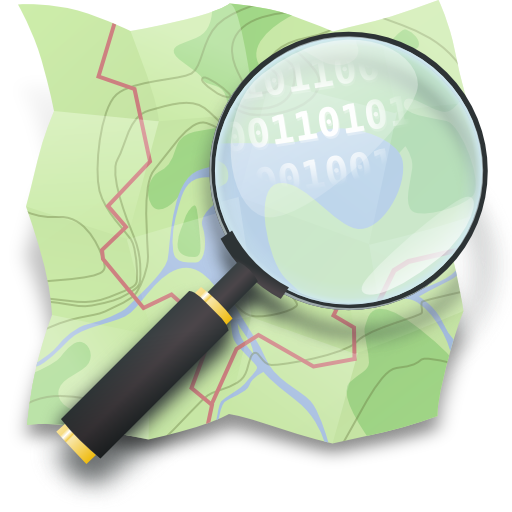
\includegraphics[width=\paperwidth,
%height=0.8\paperheight]{mag_map.png}
%}

\begin{document}

%\maketitle

\begin{frame} 


\begin{figure}
  \centering
  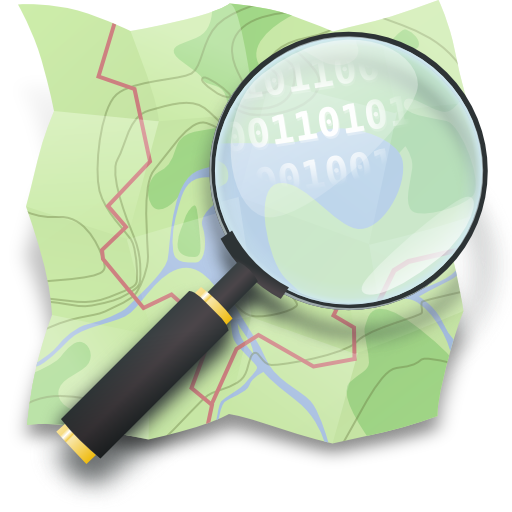
\includegraphics[width=.5\textwidth]{mag_map.png}
\end{figure}

\begin{center}
\Huge{OpenStreetMap\\}
\end{center}

\begin{center}
\Large{\emph{Die freie Wiki-Weltkarte}}
\end{center}

\end{frame}



\begin{frame}{Vorstellung}

  \begin{itemize}
    \item Michael Maier \textless \href{mailto:Michael.Maier@student.tugraz.at}{Michael.Maier@student.tugraz.at}\textgreater
    \item Telematik-Student an der TU Graz 
    \item OpenStreetMap seit Juli 2010
    \item Leite den Grazer Stammtisch seit May 2011
    \item Vorträge, Workshops und Auftragsarbeiten rund um OpenStreetMap
%    \begin{itemize}
%      \item OSM-username: \emph{\href{http://www.openstreetmap.org/user/species}{species}}
%      \item Mapping-area Graz, Leoben on bicycle, motorbike or on public transport
%    \end{itemize}
  \end{itemize}
\end{frame}

\section{Einleitung}

\begin{frame}{Was ist OpenStreetMap}

\begin{itemize}
  \item OpenStreetMap (OSM) ist eine freie Weltkarte nach dem Wiki-Prinzip
  \begin{itemize}
    \item \emph{Eigentlich eine Geo-Datenbank}
  \end{itemize}
  \item Entsteht aus der Arbeit von \textgreater 1\,M Hobbykartografen ``\emph{Mapper}''
  \item Das komplette ``planet file'' ist ca. 390\,GB groß (xml)
  \begin{itemize}
    \item 1.819.150.681 Nodes
    \item 174.489.783 Ways
    \item 1.862.942 Relations
  \end{itemize}

\end{itemize}

\end{frame}


\begin{frame}{Warum OpenStreetMap?}

Wir brauchen freie Geodaten!

\pause
\vspace{2mm}
Vorhandene Geodaten 
\begin{itemize}
  \item	für kommerzielle Nutzung zu teuer
  \item	wenn es sie denn gibt - zB Haiti
  \item	gratis nur für Lehre und Forschung
\end{itemize}

\pause
\vspace{2mm}
Karten kommerzieller Anbieter nur sehr restriktiv nutzbar
\begin{itemize}
  \item Restriktive Lizenzen - only Free as in Beer
  \item Offline-Nutzung oft nicht erlaubt - Roaming!
  \item Absichtliche Fehler, Änderungen/Richtigstellungen?
%  \pause
%  \item Bsp Google TOS: Durch die Nutzung schließen sie einen rechtsgültigen Vertrag mit Google - Dürfen unmündige Personen (unter 18?) Google Maps überhaupt nutzen?
%  \item Kosten! Google verlangt ab 25K API-Zugriffen/Tag!
\end{itemize}

\end{frame}


\begin{frame}{Wer steckt hinter OpenStreetMap?}
  \begin{itemize}
    \item OpenStreetMap Foundation (Server, Rechtliche Vertretung)
      \pause
    \item Mapper ($\sim$20.000 aktiv), meist Freiwillige ohne Geo-Hintergrund
    \begin{itemize}
      \item Lokale Mapper: OSM in Gegenden mit aktiver Community gut
      \item Jährliche Konferenz - Die \emph{State of the Map} - heuer vom 6.-8. September im Birmingham
    \end{itemize}
      \pause
    \item Universitäten
    \begin{itemize}
      \item Bakk-, Master- und Doktorarbeiten mit OSM
      \item Server-Hosting
    \end{itemize}
      \pause
    \item Organisationen, die Daten sponsern
    \begin{itemize}
      \item Firmen wie Yahoo/Bing, die Luftbilder zur Verfügung stellen
      \item Regierungen mit besseren Open-Data-Gesetzen als Österreich
    \end{itemize}
      \pause
    \item Firmen, die mit OSM arbeiten
    \begin{itemize}
      \item Geofabrik (de)
      \item MapQuest (us)
      \item BikeCityGuide (Graz)
    \end{itemize}
  \end{itemize}

\end{frame}
%\section{Introduction}




% \begin{frame}{What is OpenStreetMap}
% 
% \begin{itemize}
%   \item OpenStreetMap (OSM) is a free world map based on the 'Wiki'-principle
%   \begin{itemize}
%     \item \emph{Technically, it's a spatial database and not a map}
%   \end{itemize}
%   \item Based on the work of \textgreater 1\,M hobbyist cartographers ``\emph{Mappers}''
%   \item The complete ``planet file''  contains 386 \,GB of data (xml)
%       \pause
%   \item Licence: Open Database Licence: Think of Creative Commons for Data.
% \end{itemize}
% 
% \begin{center}
% 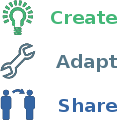
\includegraphics[width=1cm]{ODbL.png}
% \hspace{2cm}
% \includegraphics[width=1.5cm]{cc-by-sa.png}
% \end{center}
% 

%\end{frame}

% \begin{frame}{Who is behind OpenStreetMap?}
%   \begin{itemize}
%     \item OpenStreetMap Foundation (servers, legal stuff)
%       \pause
%     \item Users ($\sim$20.000 active monthly), most with little technical background
%     \begin{itemize}
%       \item Local communities - OSM is strong where the communities are
%       \item Yearly Conference - The State of the Map
%     \end{itemize}
%       \pause
%     \item Universities
%     \begin{itemize}
%       \item Bsc, Msc, PhD-Thesis with OSM
%       \item Server-Hosting
%     \end{itemize}
%       \pause
%     \item Organisations that sponsor data:
%     \begin{itemize}
%       \item Companies like Yahoo, Bing allow use of aerials for tracing
%       \item Goverments with Open Data portals
%     \end{itemize}
%       \pause
%     \item Organisations that work with OSM Data:
%     \begin{itemize}
%       \item geofabrik.de
%       \item MapBox
%       \item MapQuest
%       \item Skobbler
%       \item BikeCityGuide
%     \end{itemize}
%   \end{itemize}
% 
% \end{frame}
% 

{
 \usebackgroundtemplate{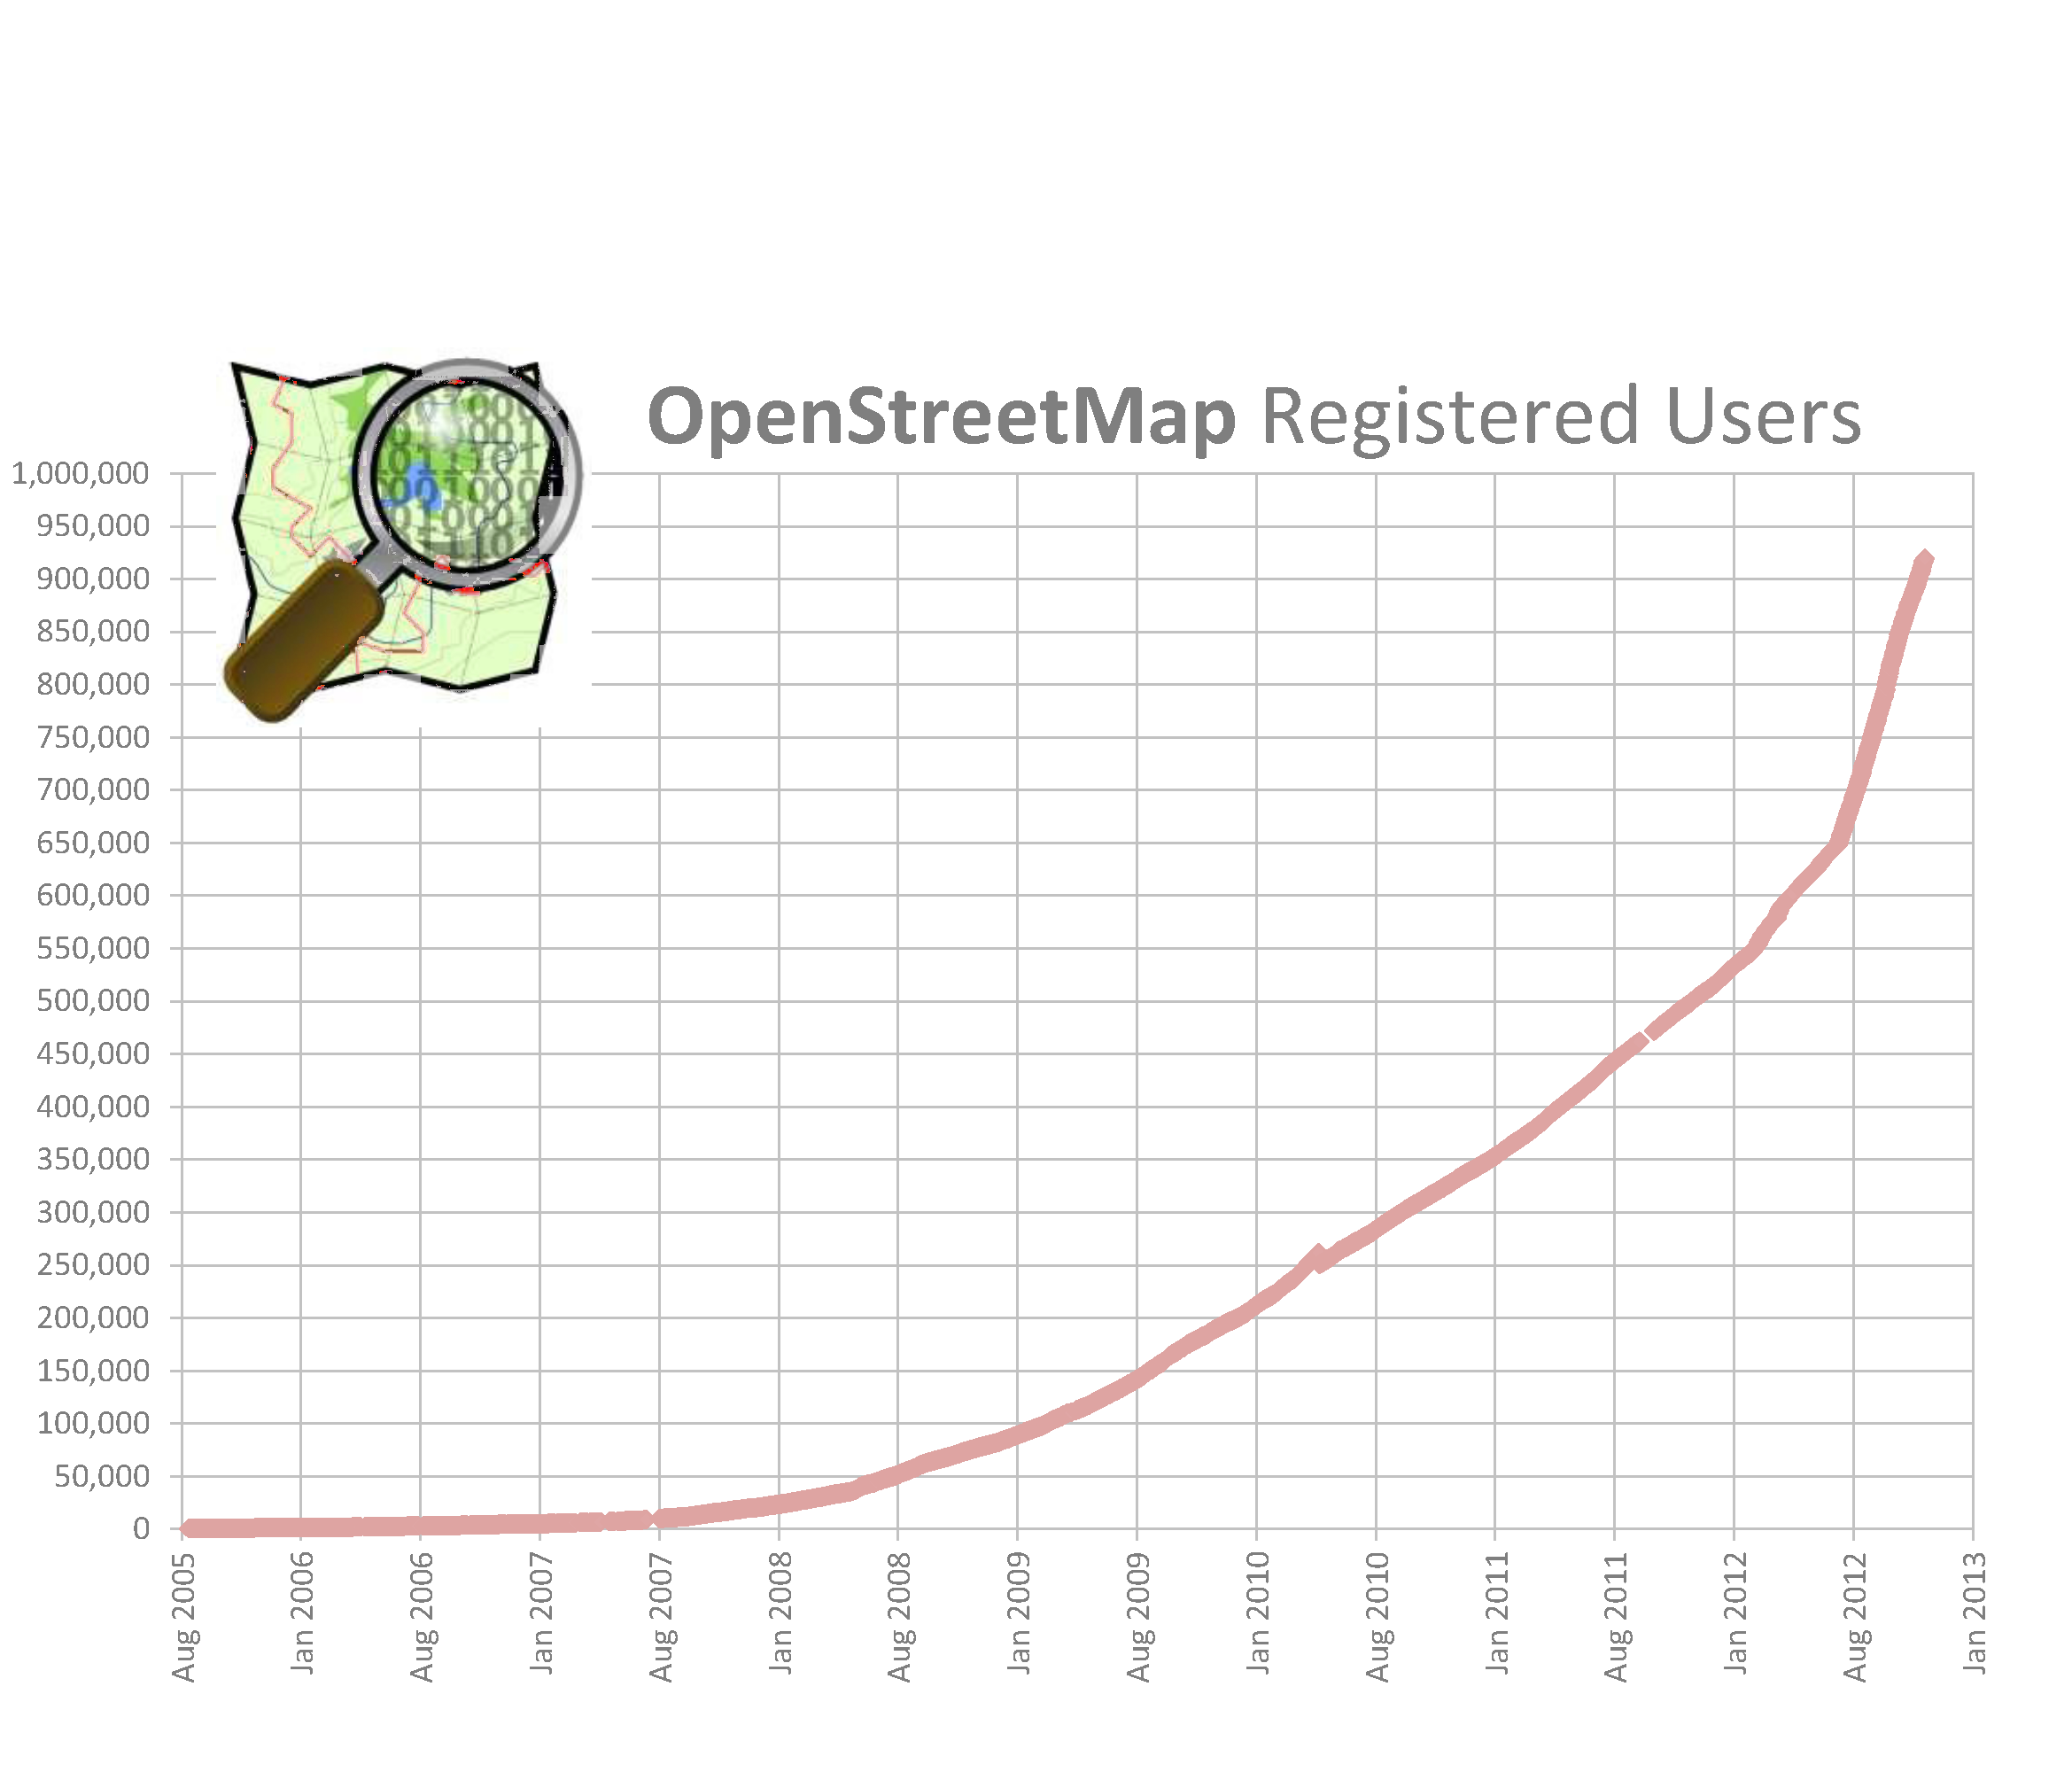
\includegraphics[width=\paperwidth]{Osmdbstats2.png}}

\begin{frame}{Geschichte}


\vspace{2cm}

\begin{itemize}
  \item Start des Projekts im August 2004 durch \emph{Steve Coast}
  \item Dezember 2006 - Yahoo erlaubt abzeichnen
  \item Juli 2007 - Erste Konferenz, ``State Of The Map 2007''
  \item August 2007 - 10,000 Registrierte Benutzer
  \item März 2009 - 100,000 Registrierte Benutzer
  \item Januar 2010 - Haiti--Projekt
  \item November 2010 - Bing erlaubt abzeichnen
  \item Juli 2011 - Erste ``State Of The Map Europe'' in Wien
  \item Gestern - 1.077.025 Registrierte Benutzer
\end{itemize}


\end{frame}

}

% 
% {
%  \usebackgroundtemplate{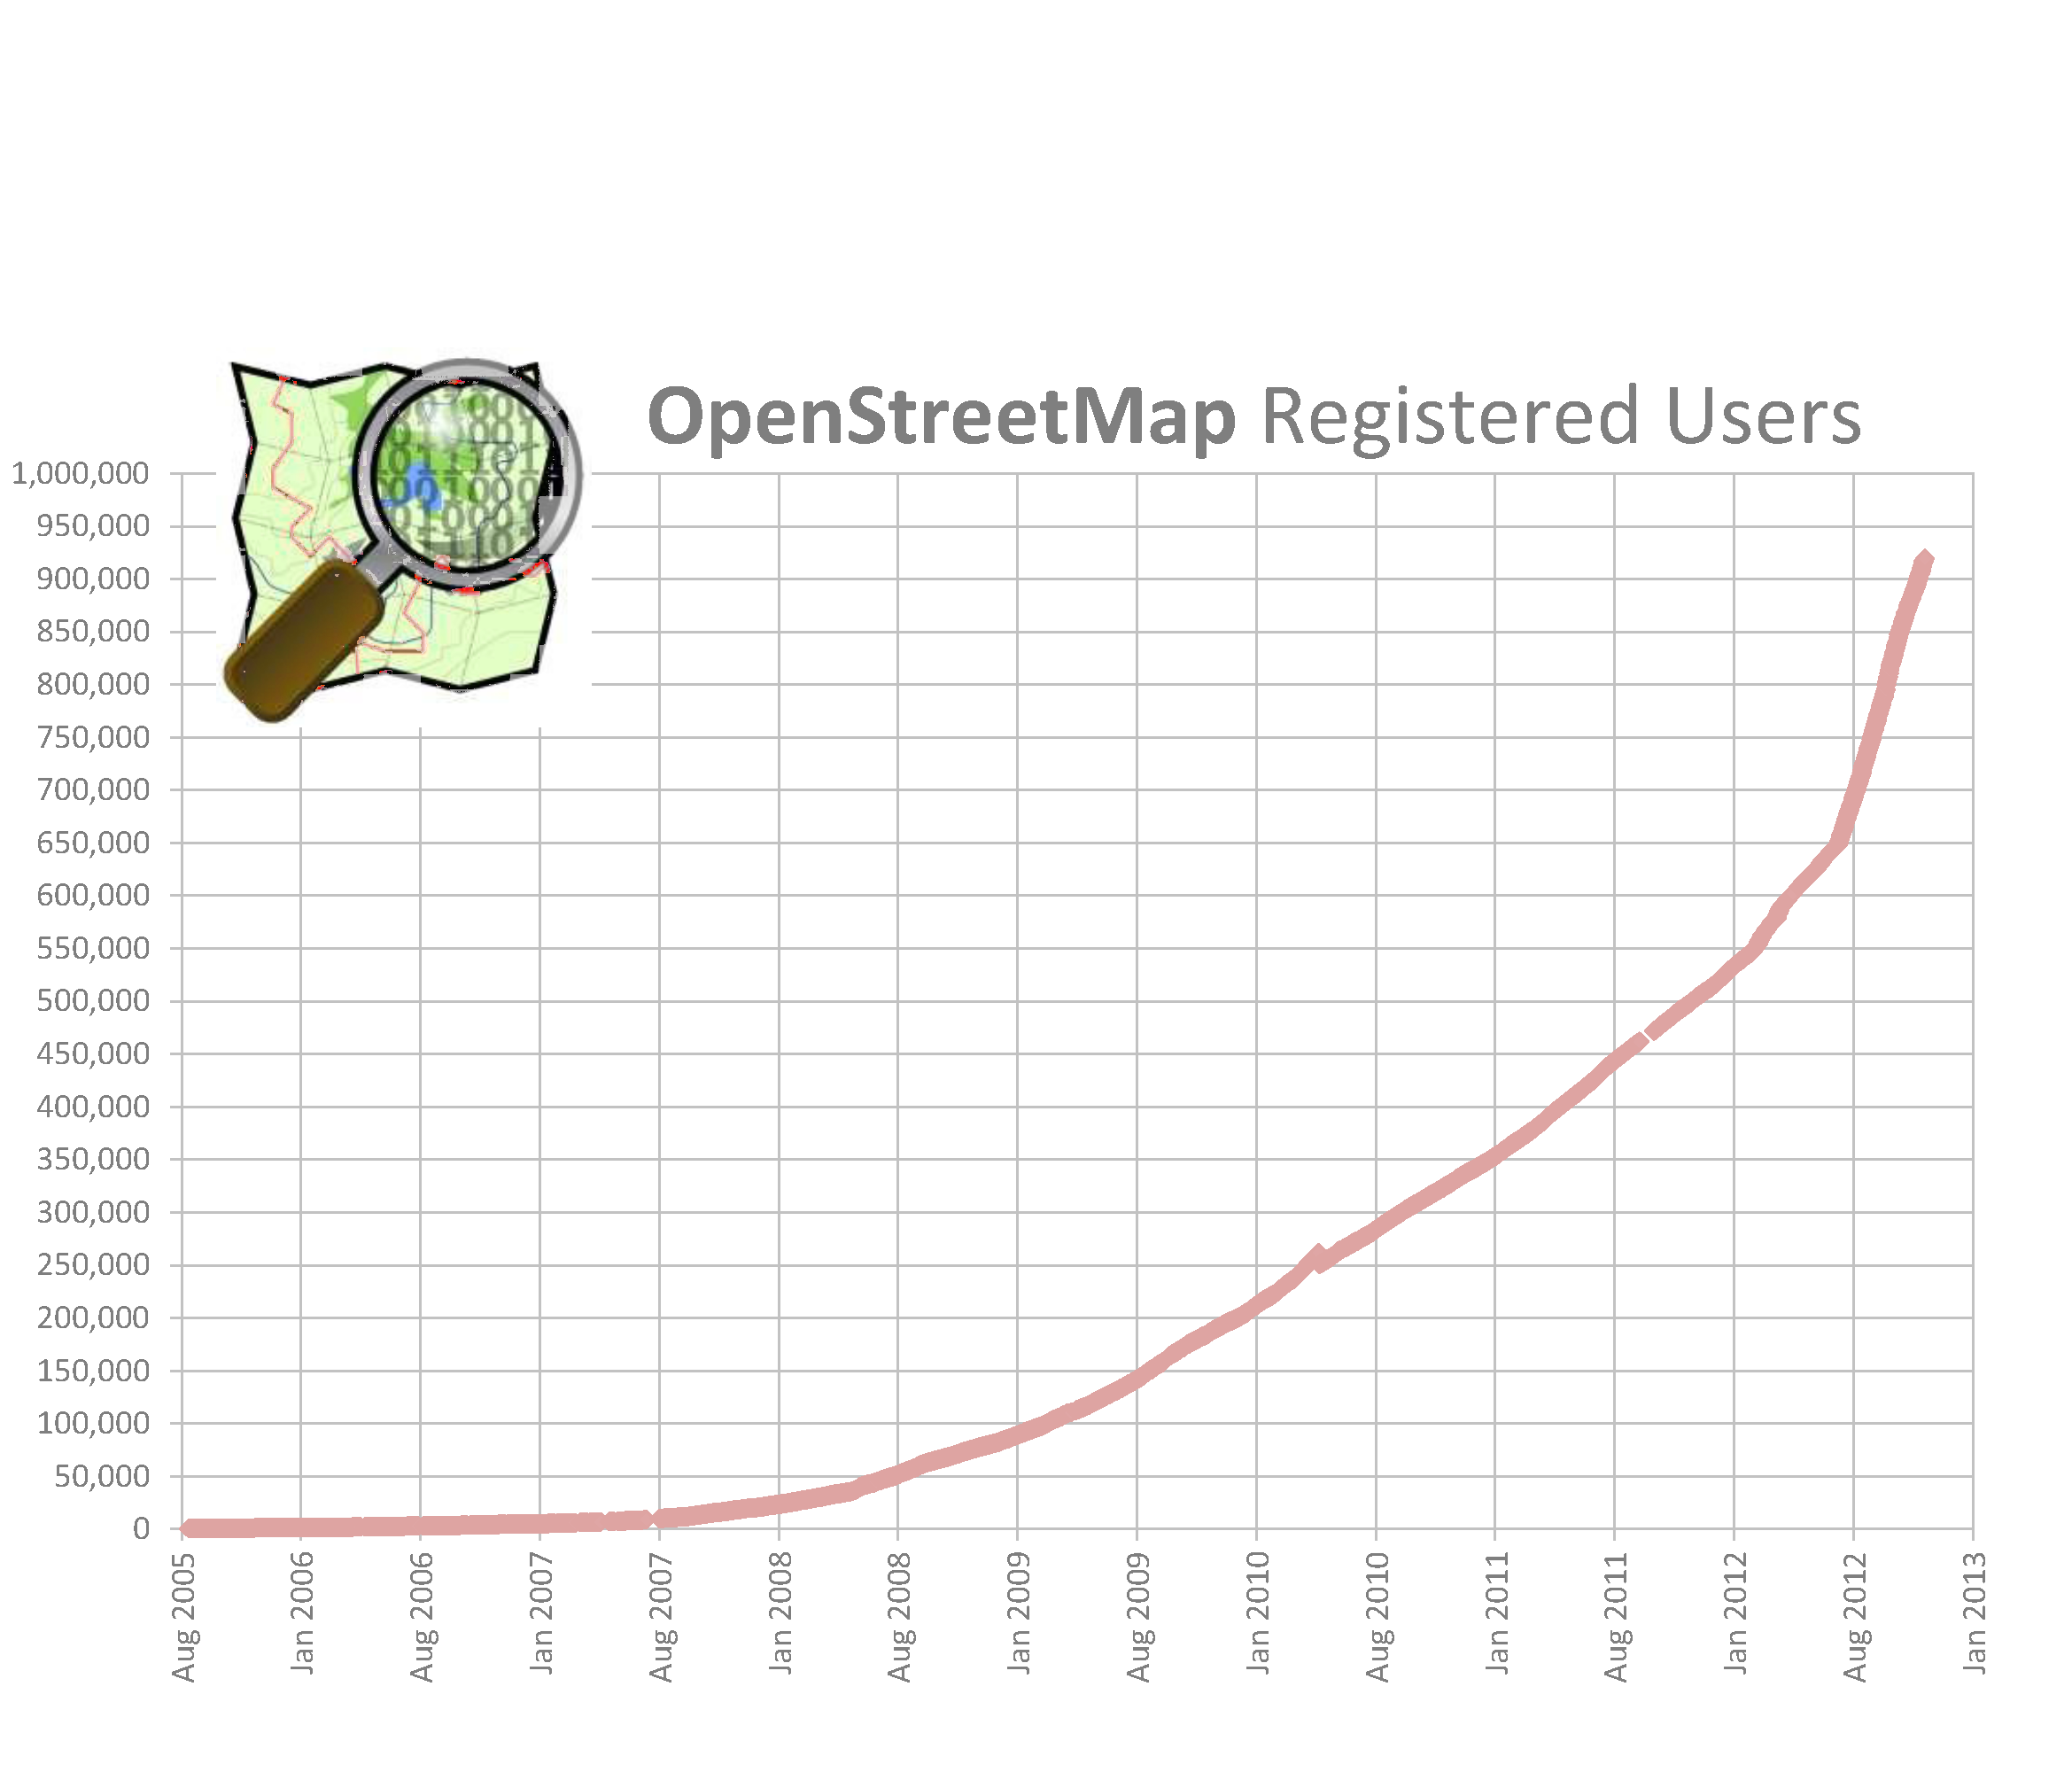
\includegraphics[height=10cm]{Osmdbstats2.png}} 
% 
% \begin{frame}{History of OSM}
%   \vspace{1.2cm}
% \begin{itemize}
%   \item Start in August 2004 through \emph{Steve Coast}
%   \item Dec. 2006 - Yahoo allows tracing
%   \item July 2007 - first conference ``State Of The Map 2007''
%   \item Aug. 2007 - 10,000 registered users
%   \item Mar. 2009 - 100,000 registered users
%   \item Jan. 2010 - 200,000 registered users - Haiti--Project
%   \item Nov. 2010 - Bing allows tracing
%   \item Nov. 2011 - 500,000 registered users
%   \item Yesterday - 1,023,125 registered users
% \end{itemize}
% 
% \end{frame}
% 
% \begin{frame}{History of OSM}
%   \vspace{1.2cm}
%   Exponential growth, 
% \begin{itemize}
%    \item 2013: 1\,M
% \end{itemize}
%   Double each 18\,month: 
% \begin{itemize}
%      \pause
%    \item 2016: 4\,M
%      \pause
%    \item 2022: 64\,M
%      \pause
%    \item 2034: 1,024\,M
%    \item ...here it gets unrealistic --- but we hope for 1/100 of the population :-)
% \end{itemize}
% 
% \end{frame}
% }
% 
% 
% \section{Why OpenStreetMap}
% 
% \begin{frame}{Why OpenStreetMap?}
% 
%   There is Google Maps...\pause Ugh!
% 
% \begin{itemize}
%   \item We need a source for free geoDATA, not only web maps!
%   \item We need to create maps with different styles, not the only one Google offers us!
%   \item We want to do routing with our own algorithms
%   \begin{itemize}
%     \item Bicycle routing that actually works
%     \item Rollerskate routing
%     \item Wheelchair routing
%   \end{itemize}
%     \pause
%   \item And all of that offline, without Internet access!
% \end{itemize}
% 
% \end{frame}
% 
% \begin{frame}{Why OpenStreetMap?}
% 
%   If you think: Fine, but I only need a web map... \pause think harder:
% 
% \begin{itemize}
%   \item What abount errors in the map? \pause HGV's get routed through my backdoor!
%   \item But MapMaker... \pause Your changes must be approved and all data you enter now belongs to Google - you NEVER get it back!
%     \pause
%   \item In Austria, using Google is illegal if you're under 18...
%     \pause
%   \item Costs! Google charges from 25\,K API calls/day onward!
% \end{itemize}
% 
% \end{frame}
% 
% \begin{frame}{Why OpenStreetMap?}
% 
% Benefits of OpenStreetMap:
% 
% \begin{itemize}
%   \item Raw data is provided
%   \item Everyone can improve the data (wiki-principle)
%   \item You can get free data for your satnav
% \end{itemize}
% 
% Freedom creates possibilities!
% 
% \end{frame}
 
\section{Wie funktioniert OpenStreetMap?}

    
\begin{frame}{Technischer Hintergrund}

Es gibt eine zentrale Datenbank (PostgreSQL/PostGIS) für Schreibzugriffe (in GB).\\
\pause
Diese wird weltweit gespiegelt für Lesezugriffe mit unterschiedlichen Methoden:

\begin{itemize}
  \item API-Lesezugriffe werden über mehrere Spiegel-Server lastverteilt
  \item Rendering-Server nutzen eine lokale, minütlich aktualisierte Datenbank
  \item Extrakte zum Download siehe \href{http://wiki.osm.org/Planet}{wiki.osm.org/Planet}
  \item Für räumliche SQL-Abfragen: Overpass API, zB alle italienischen Restaurants in Graz
\end{itemize}

\end{frame}

\begin{frame}{Datenmodell}

Wurde von Informatikern ohne Geo-Vorbelastung erstellt:
\begin{itemize}
  \item Punkte (Koordinaten), $\Rightarrow$ ``Node'' 
\includegraphics[width=0.5cm]{node.png}
	\begin{itemize}
          \item POIs
\pause
\item Teile von Wegen
\end{itemize}
  \item Linienzüge sind eine Reihe von Nodes, $\Rightarrow$ ``Way'' 
\includegraphics[width=0.5cm]{way.png}
	\begin{itemize}
	  \item Wege, Flüsse, Hecken etc.
	\item können geschlossen sein: Gebäude, Flächen
\end{itemize}
\pause
  \item Gruppierungen von Ways/Nodes $\Rightarrow$ ``Relations'' 
\includegraphics[width=0.5cm]{relation.png}
	\begin{itemize}
          \item Streckenrelationen, zB ÖPNV-Routen, Radrouten
	\item Multipolygone (Zusammengesetzte Flächen mit Ausschnitten)
	\item Abbiegebeschränkungen (Way:von, Way:nach, Node:über)
	\item Meta-Relationen, zB für Verkehrsverbünde
	\end{itemize}
\end{itemize}

\end{frame}

\begin{frame}{Datenmodell 2}

Jedes Element kann Eigenschaften $\Rightarrow$ ``Tags'' haben, zB:
\begin{itemize}
  \item amenity = cafe 
\includegraphics[width=0.5cm]{cafe.png}
  \item highway = footway 
\includegraphics[width=1cm]{footway.png}
  \item building = yes  
\includegraphics[width=0.5cm]{building.png}
  \item landuse = farmland
\end{itemize}

Tags sind Freitext, beliebige Anzahl!

Standards werden im Wiki festgelegt, siehe \href{http://wiki.openstreetmap.org/wiki/DE:How\_to\_map\_a}{wiki/DE:How\_to\_map\_a}

\vspace{4mm}
\pause
\begin{itemize}
  \item Koordinaten sind in Dezimalgrad, WGS84. 
	\begin{itemize}
  \item 3D-Information werden als Tags eingetragen, zb ele=435
\end{itemize}
  \item Genauigkeit 7 Stellen, entspricht 1\,cm am Äquator.
  \item Standard-Dateiformat: XML
\end{itemize}

\end{frame}

\begin{frame}{Lizenz}

Die Daten stehen unter der Open Database Licence - Entspricht etwa Creative Commons - Attribution - Sharealike für Daten.
\begin{itemize}
  \item Jeder darf die Daten, auch kommerziell verwenden
  \item Quelle: ``OpenStreetMap and Contributors, ODbL'' muß angegeben werden.
\end{itemize}

 \begin{center}
 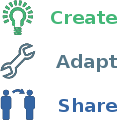
\includegraphics[width=1cm]{ODbL.png}
 \hspace{2cm}
 \includegraphics[width=1.5cm]{cc-by-sa.png}
 \end{center}

\pause
Die Web-karten (gerenderten Tiles) auf \href{http://osm.org}{openstreetmap.org} sind CC-BY-SA, beachte \href{http://wiki.openstreetmap.org/wiki/Tile\_usage\_policy}{Tile Usage Policy}!

\end{frame}

\begin{frame}{Qualitätssicherung}

Wie ein Wiki, jeder darf alles ändern!\\
\pause
Jedoch konfliktfreier als bei Wikipedia, da:
\begin{itemize}
  \item Geodaten die Realität abbilden, nicht Meinungen von Menschen
  \item Jeder Mapper kann persönlich via Message-System kontaktiert werden
	\begin{itemize}
	  \item Diskussion über die Mailingliste
	\end{itemize}
\pause
  \item Automatische Qualitätssicherungs-Werkzeuge
\begin{itemize}
  \item \href{http://keepright.ipax.at/report\_map.php?zoom=14&lat=48.20808&lon=16.37221}{keepright.ipax.at}
  \item \href{http://openstreetbugs.org}{openstreetbugs.org}
\end{itemize}

\end{itemize}

\end{frame}

\section{Wie OpenStreetMap nutzen?}

\begin{frame}{Interaktive Web-Karten}

Hauptseite: \href{http://osm.org}{www.OpenStreetMap.org}

\vspace{7mm}

Spezialkarten:
  \begin{table}[htbp]
    \centering
    \begin{tabular}{r|l}
      Radkarte  &  \url{http://opencyclemap.org} \\
      Wanderkarte & \url{http://hikebikemap.de} \\
      Rauchfrei-Karte & \url{http://OpenGastroMap.org} \\
      Rollstuhl-Karte & \url{http://wheelmap.org} \\
      Seekarte & \url{http://OpenSeaMap.org} \\
\pause
      200 weitere: & siehe \href{http://wiki.openstreetmap.org/wiki/List\_of\_OSM\_based\_Services}{OSM-Wiki} \\
%      Interaktive Informationskarte & http://openstreetbrowser.org
    \end{tabular}
  \end{table}

Blitzschnelles Routing: \url{http://osrm.at}

\end{frame}

\begin{frame}{Arbeiten mit OSM-Daten}

OSM-Daten direkt auf osm.org downloaden - Tab ``Export'' $\Rightarrow$ OpenStreetMap XML Data

\pause
\vspace{8mm}
Wie bekommt man den kompletten Planet?

\begin{itemize}
  \item Extrakte siehe \href{http://wiki.osm.org/Planet}{wiki.osm.org/Planet}
  \begin{itemize}
    \item .dbf - binary file format, effizient komprimiert
    \item .osm.xml - Standard OSM Format
    \item ESRI Shapefile (ausgewählte Spalten)
  \end{itemize}
\end{itemize}

\end{frame}

\begin{frame}{Arbeiten mit OSM-Daten 2}

Wie OSM-Daten in die eigene GIS-Datenbank (Postgres/PostGIS) spielen?
\begin{itemize}
  \item Download der Extrakte
  \item Zuschneiden mittels \href{http://wiki.openstreetmap.org/wiki/Osmosis}{Osmosis} (Java)
  \item Importieren mittels \href{http://wiki.openstreetmap.org/wiki/Osm2pgsql}{Osm2pgsql} (Python, Windows/Linux)
	\begin{itemize}
	  \item Spaltenauswahl mittels Konfigurationsdatei
	\end{itemize}

  \item Öffnen mittels \href{http://www.qgis.org}{Quantum GIS}

	\begin{itemize}
	  \item Exportieren als Shapefile
	\end{itemize}

\end{itemize}

\end{frame}


% \section{How to use OpenStreetMap}
% \subsection{Use OpenStreetMap}
% 
% \begin{frame}{Use OSM Services Directly}
% \begin{columns}[c] % the "c" option specifies center vertical alignment 
% \column{.3\textwidth} % column designated by a command
%   \url{www.osm.org}\\
% 
%   \begin{itemize}
%     \item Search (Nominatim)
%     \item 4 different map styles
%     \item View history of areas/objects
%     \item Data display
%     \item Edit with Potlatch (Flash)
%   \end{itemize}
% 
% \column{.7\textwidth} 
% 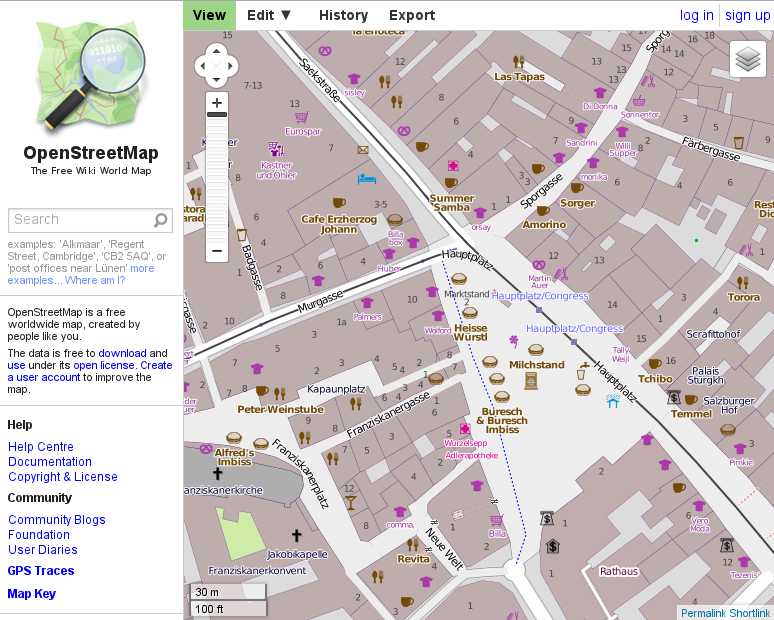
\includegraphics[width=.65\paperwidth]{osm.png}
% \end{columns}
% \end{frame}
% 
% \begin{frame}{Websites Showing Special Data}
% 
% OpenStreetMap is not only about its main page, most of its value is generated through other maps generated from its data:
% 
% \begin{itemize}
%   \item \href{http://www.openseamap.org/}{OpenSeaMap}
%   \item \href{http://wiki.openstreetmap.org/wiki/Wheelmap}{Wheelmap}
%   \item Cuisine in Restaurants: \href{http://www.opengastromap.de/?lat=47.07&lon=15.43&zoom=12}{opengastromap.de}
%   \item Smoker's Map: \href{http://toolserver.org/~stephankn/smoking/}{opengastromap.org}
%     \pause
%   \item for \textgreater200 more, see the \href{http://wiki.openstreetmap.org/wiki/List\_of\_OSM\_based\_Services}{OSM-Wiki}
% \end{itemize}
% \end{frame}
% 
% \begin{frame}{Routing:}
% 
% 
% \begin{itemize}
%   \item \url{OpenRouteService.org} (+pedestrian, bike with profiles)
%   \item \url{maps.cloudmade.com} (+bike, pedestrian)
%   \item \href{http://osrm.at/2eq}{Open Source Routing Machine} car only, but VERY fast.
% \end{itemize}
% The whole ist of routing services based on OSM is available at \url{http://wiki.osm.org/Routing/OnlineRouters}
% \end{frame}
% 
% \begin{frame}{Mobile Apps}
%   The future: Ubiquitous Computing!
%   
%   \pause
% 
%   Apps using OpenStreetMap on:
% 
% \begin{itemize}
%   \item  Android ( \textgreater 70) \url{http://wiki.osm.org/Android}
%   \item  iPhone ( \textgreater 60 )  \url{http://wiki.osm.org/Apple\_iOS}
%   \item  Blackberry ( 8 ) \url{http://wiki.osm.org/BlackBerry\_OS}
% \end{itemize}
% 
% Of course, you can use OSM on your Garmin, see \href{http://wiki.osm.org/Garmin}{wiki.osm.org/Garmin}!
% 
% \end{frame}
% 
% 
% \begin{frame}{Download OSM Data}
% 
% You can use the ``Download''-button on osm.org - for small areas
% 
% \pause
% I want the whole planet!
% 
% \begin{itemize}
%   \item Excerpts for download see \href{http://wiki.osm.org/Planet}{wiki.osm.org/Planet}
%   \begin{itemize}
%     \item .dbf - binary file format, efficient compressed
%     \item .osm.xml - standard OSM format
%     \item ESRI Shapefile
%   \end{itemize}
% \end{itemize}
% \end{frame}
% 
% 
% \begin{frame}{Creating You Own Map}
% 
%   Its now very easy thanks to the new Overpass API. All you need is a short snipplet of JavaScript. Background and data are served from OpenStreetMap!
% 
%   Some examples:
% 
%   \begin{itemize}
%     \item A \href{http://maxheight.bplaced.net/overpass/prototyp.html?zoom=14&lat=50.7322&lon=7.09816&layers=B0000000TFFFFFFFFFFFTTT&label=T&opacity=70}{Maxheight Map} 
%     \item A map themed around \href{http://mijndev.openstreetmap.nl/~ligfietser/fiets/?map=cycleways&zoom=15&lat=47.07201&lon=15.43873&layers=B00000FFFFFFTTFTFTFFFFF}{Bicycles}
%     \item Of course OSM supports \href{http://map.comlu.com/}{Turn Restrictions}!
%     \item More sophisticated: \href{http://simon04.github.com/POImap/ivb.html}{Public Transport Map} of Innsbruck
%     \item \dots
%     \item Create your own: \href{http://overpass-turbo.eu/?q=PCEtLQpUaGlzIMSHIGFuIGV4YW1wbGUgT3ZlcnBhc8SIcXXEmXkuxIRyecSJdCBvdcSoYsSmcHJlxJ1pbmcgdGjElVJ1xI1ixKt0b8SNYWJvxJghClnEqiBjxIwgZsSzZCBtb8SwxI7EkMSSxJTEiHdpxLfEtsS4IExvYcWQxL9vbMSjxII-CjzEn8ShxLZ5cGU9Im5vZGUixakgIDxoxJwta3Yga8WyxJFlbsWbeSIgdsWyZHLEs2vEs2dfd2F0xJkiL8W5xbtixYN4LcWsxKUge3vGnW94fX3GmsSAxILEt8SKxIphxKtvLWNvxZdlxpfFkMWaxZzEt2UKxbrHgMeBx4LHgmN1csSwbsSobWFwxotpZXfFim\_Fk2TEs8aWxLEuxajFqi\_GoXnFqTzEr8SzdMaa&c=BOxHDJTqUR&R}{overpass-turbo.eu}
%   \end{itemize}
% 
%   
% \end{frame}
% 
  \subsection{ OpenStreetMap Verbessern}

\begin{frame}{Editing}

  Eine große Auswahl an Editoren steht fürs Web, Desktop- und Mobilnutzung zur Verfügung

  \begin{itemize}
    \item Web:
    \begin{itemize}
      \item Potlatch (Flash)
      \item JOSM web-start
      \item iD (JavaScript), in development
    \end{itemize}
    \item Mobile (Auswahl): Alle siehe  \href{http://wiki.openstreetmap.org/wiki/Android\#OpenStreetMap\_editing\_features}{Android}, \href{http://wiki.openstreetmap.org/wiki/Apple\_iOS\#OpenStreetMap\_editing\_features}{iOS}:
    \begin{itemize}
      \item Vespucci: Ausgewachsener Editor
      \item osmaptuner: Existierende POIs ergänzen
      \item OsmTracker: GPS-Tracks, Audio, Schnell POIs hinzufügen
    \end{itemize}
  \item Desktop
    \begin{itemize}
      \item \href{http://josm.openstreetmap.de}{JOSM} (Java)
      \item \href{http://merkaartor.be}{Merkaartor} (C++)
      \item \href{http://www.qgis.org/}{Qgis} (C++)
      \item ArcGIS in neuester Version 10.1
    \end{itemize}
  \end{itemize}

\end{frame}

% \section{How does OSM work?}
% 
% \begin{frame}{Understanding the Data(base)}
%   OSM is a geospatial database with three basic elements:
% 
%   \begin{itemize}
%     \item Nodes: Defined through x,y coordinates 
\includegraphics[width=0.5cm]{node.png}
%     \item Ways: a string of nodes 
\includegraphics[width=0.5cm]{way.png}
%     \item Relations: A meta ``Group'' that can include Nodes and Ways 
\includegraphics[width=0.5cm]{relation.png}
%   \end{itemize}
% 
%   \pause
% 
%   Each of these basic elements can have properties $\Rightarrow$ ``Tags'', e.g.:
%   \begin{itemize}
%     \item amenity = cafe 
\includegraphics[width=0.5cm]{cafe.png}
%     \item highway = footway 
\includegraphics[width=1cm]{footway.png}
%     \item building = yes  
\includegraphics[width=0.5cm]{building.png}
%     \item landuse = farmland 
%   \end{itemize}
% 
%   These properties are free textfields written as key=value pair.
% 
% \end{frame}
% 
% \begin{frame}{Understanding the Data(base) 2.}
%   
%   So, what do we tag?
%   \pause
%   Everything!
% 
% \begin{itemize}
%   \item highway=*, landuse=*, shop=*, tourism=*, 
%   \item e.g. amenity=restaurant, cuisine=pizza, smoking=no, wheelchair=yes, ...
%   \item ?=*
% \end{itemize}
% 
% Althrough free text, common standards have been worked out in the Wiki.
% 
% $\Rightarrow$ all relevant tags can be found in the Wiki!
% 
% \end{frame}
% 
% 
%     
% \begin{frame}{Technical Background}
% There is 1 central Database (postgres/postgis) for writes (located in GB)\\
% This DB is mirrored all over the world for reads with different methods:
% 
% \begin{itemize}
%   \item Rendering servers use a minutely updated local DB
%   \item API read calls are load-balanced over multiple readonly servers
%   \item Excerpts for download see \href{http://wiki.osm.org/Planet}{wiki.osm.org/Planet}
%   \item overpass API for VERY fast SQL-like calls directly on a DB, e.g. give me all pubs in Graz
% \end{itemize}
% 
% \end{frame}
% 
% 
% \section{How to use OpenStreetMap}
% 
% \begin{frame}{Future Possibilities}
% 
%   What are the possibilities of an open geo database like OSM?
%   \pause
%   Endless!
% 
% Ubiquitous computing needs to know its surroundings!
%   \begin{itemize}
%     \item Where am I?
%     \item What is nearby?
%   \end{itemize}
% 
%   $\Rightarrow$ A geospatial database is needed for Ubiquitous Computing!
% 
% \end{frame}
% 
% \begin{frame}{What Tags in OSM are useful?}
%   Especially people with disabilities need special routing instructions:
%   \begin{itemize}
%     \item Is there a tactile paving on the way
%     \item crossings:
%     \begin{itemize}
%       \item Number of lanes to cross
%       \item traffic\_signals:sound ?
%       \item traffic\_signals:arrow ?
%       \item traffic\_signals:minimap ?
%     \end{itemize}
%     \item surface type: asphalt, cobblestone, grass
%     \item are there lowered kerbs?
%   \end{itemize}
% \end{frame}
% 
% 
% \begin{frame}{A Routing example}
% 
%   E.g. A user asks his mobile assistant Siri: Where is the nearest italian restaurant?
% 
%   Lets imagine Siri knows the following information:
%   \begin{itemize}
%     \item Where is the user? Currently in Tram~7, coordinates from Galileo.
%     \item The user is a non-smoker.
%     \item The user is a vegetarian.
%   \end{itemize}
% 
% \end{frame}
% 
% \begin{frame}{A Routing example 2.}
% 
%   \begin{itemize}
%     \item Siri queries all \emph{amenity=restaurant},\emph{cuisine=italian} POIs from OSM around 5\,km.
%     \item Only restaurants with the \emph{smoking=[no$\vert$isolated]} tag are considered.
%     \item Restaurants with the \emph{diet:vegetarian=yes} tag are preferred.
%     \item Parsing tag: \emph{opening\_hours=*} filters out closed restaurants.
%     \item It fetches the next \emph{railway=tram\_stop} points from the tram route from OSM, and starts to calculate the route from them to the POIs.
%     \item It queries the \emph{contact:phone=*} information from OSM and dials the phone number to make a reservation.
%       \pause
%     \item While on the tram, it starts raining. The route is being recalculated to include as less ways with \emph{covered=no} set as possible.
%   \end{itemize}
% \end{frame}
% 
% 
% \begin{frame}{A Today's Example}
%   \url{http://www.schau.auf.linz.at}
%   Every citizen can report defective road inventory, overfull waste bins and other annoyances.
%   \pause
%   
%   Possible today: routing considering highway=construction on a daily basis!
% 
% \end{frame}
% 
\begin{frame}{3D is the Future!}
  3D is coming to OSM! See example at \href{http://maps.osm2world.org/?zoom=17&lat=47.06156&lon=15.46983&layers=BF0FTFFF}{maps.osm2world.org}.

  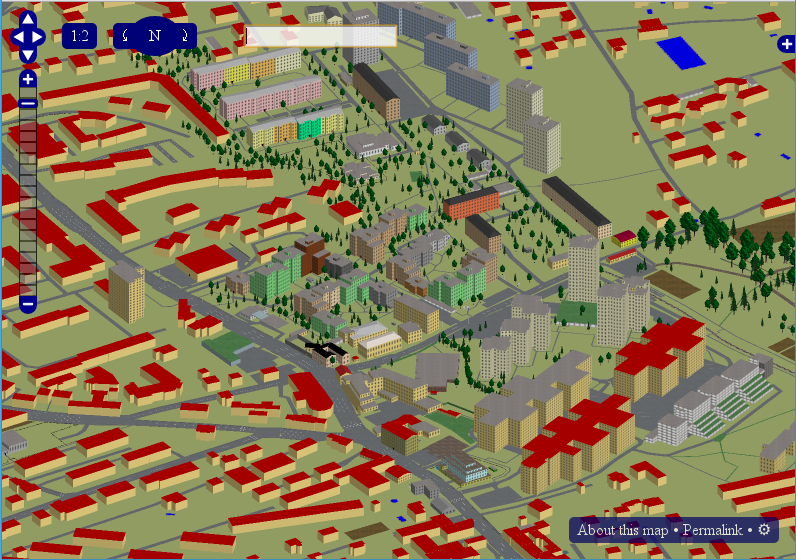
\includegraphics[width=0.9\textwidth]{3d.png}


\end{frame}
% 
% \begin{frame}{What does OSM Need in the Future?}
% 
%   OSM is ideal for any project where geodata is needed.
% 
%   OSM coverage is better in cities than commercial data providers, but we need more data everywhere!
% 
%   \begin{itemize}
%     \item Promote Open (Goverment) Data in your organisation!
%       \begin{itemize}
%         \item housenumbers are most urgent for geolocation!
%         \item public toilets, defibrillators, tree cataster
%         \item poo-bags \dots
%       \end{itemize}
%     \item Help OSM by fixing errors yourself
%   \end{itemize}
% 
% \end{frame}
% 
% 

% \begin{frame}{Help}
% 
% \begin{itemize}
%   \item First place should be the wiki:\url{http://wiki.openstreetmap.org}
%   \item For questions: $\Rightarrow$ mailing lists!
%   \pause
% \item If it exists in your town: the local user group meeting! see \href{http://usergroups.openstreetmap.de/}{Map}.
% \end{itemize}
% 
% \end{frame}
% 
\begin{frame}{Hilfe}

\begin{itemize}
  \item Erste Station sollte das Wiki sein: \href{http://wiki.openstreetmap.org}{wiki.openstreetmap.org}
  \item Immer noch etwas unklar? $\Rightarrow$ Mailingliste \href{http://lists.openstreetmap.org/listinfo/talk-at}{talk-at}
  \pause
  \item \href{http://wiki.openstreetmap.org/wiki/Graz/Stammtisch}{Stammtisch Graz} alle 2 Monate - der nächste Montag, 25.3.2013, Brot und Spiele!
\end{itemize}

\end{frame}

\section{Ende}

\begin{frame}{Vielen Dank für die Aufmerksamkeit!}

  Folien zum Geo-Kolloquium am 20.3.2013, Graz
\vspace{1cm}

Folien unter: \includegraphics[width=1cm]{cc-by-sa.png}.
\vspace{1cm}

Erstellt mittels \LaTeX Beamer, Quelltext: \href{https://github.com/species/vortrag-osm-geo-kolloquium}{Github}.
\vspace{1cm}

\href{mailto:michael.maier@student.tugraz.at}{Michael Maier}

Twitter: \href{https://twitter.com/osmgraz}{@osmgraz}
\end{frame}

\end{document}
